\documentclass[a4paper, 11pt]{article}

\usepackage[utf8x]{inputenc}
\usepackage[T1]{fontenc}
\usepackage{ucs}
\usepackage[english]{babel}
\usepackage{mathtools, amsmath, amsfonts}
\usepackage{fancyhdr}
\usepackage[parfill]{parskip}
\usepackage{graphicx}
\usepackage{palatino,newtxmath}
\usepackage{float}
\usepackage[font={small,it}]{caption}
\usepackage{fixltx2e}
\usepackage{zed-csp}
\usepackage[scaled]{helvet}
\usepackage{fullpage}
\usepackage{minted}

\linespread{1.05}
\pagestyle{fancyplain}
\fancyhead{}
\fancyfoot[L]{}
\fancyfoot[C]{}
\fancyfoot[R]{\thepage}
\renewcommand{\headrulewidth}{0pt}
\renewcommand{\footrulewidth}{0pt}
\setlength{\headheight}{13.6pt}

\setcounter{secnumdepth}{0}
\widowpenalty=1000
\clubpenalty=1000

\newcommand{\horrule}[1]{\rule{\linewidth}{#1}}

\title{ 
\normalfont \normalsize 
\textsc{University of Copenhagen} \\ [25pt]
\horrule{0.5pt} \\[0.4cm]
\huge XMP: Exam \\ \Large - Programming \\
\horrule{2pt} \\[0.5cm]
}

\author{Jens Fredskov (chw752)}

\begin{document}
\maketitle
\pagebreak

\section{Implementation} % (fold)
\label{sec:implementation}
The implementation consists of several different processes, in addition to a few helper functions, types and data structures. The processes largely communicate as outlined in Figure \ref{fig:simulation}.
\begin{figure}[H]
    \centering
   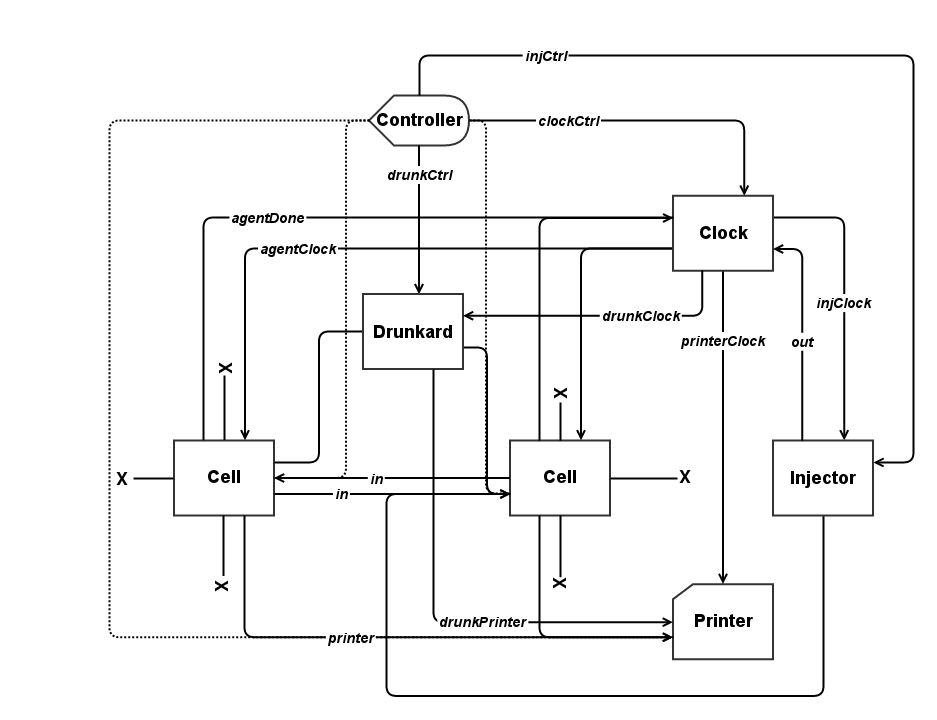
\includegraphics[width=1\textwidth]{pedestrian_simulation.png}
   \caption{Communication between the processes of a pedestrian simulation. Here only two cells are shown, to keep the figure clearer. The dotted lines indicate that the controller only holds these channels for the purpose of closing them in the exit phase.}
\label{fig:simulation}
\end{figure}
As can be seen from the figure the pedestrians themselves are not a process. These are instead data passed between the other processes on their respective channels. In general the communication of the implementation is as follows.

\paragraph{Cell} % (fold)
\label{par:cell}
A cell starts by waiting for messages from other cells, injectors and drunkards. When it receive such a message it will respond whether it has accepted the pedestrian, or drunk, in the message or not. It it only declines if it already has a pedestrian or a drunk. When a cell holds a pedestrian it will also wait for the clock to send a tick, after which it will try to send the pedestrian to on of its neighbors. If the cell has no neighbor in a direction it tries to send, it will instead let the pedestrian walk off the board and inform the clock that one less pedestrian exists. The cell also informs the printer each turn when it has a pedestrian. If the cell receives a drunk, it will not try to move it, but instead only decline on its input channel, until the drunkard process informs the cell that the drunk has moved, after which the cell is back to its original state.
% paragraph cell (end)

\paragraph{Injector} % (fold)
\label{par:injector}
The injector waits on input from either the clock or the controller. If it receives a tick from the clock it will check whether it should inject a pedestrian, and if so try to do this. If the cell it tries to inject at declines, i.e. it is occupied, the injector simply skips the injections this turn. The injector then informs the clock whether or not an extra pedestrian now exists on the board. If the injector receives a input from the controller it will change its injection rate to the one it has received.
% paragraph injector (end)

\paragraph{Clock} % (fold)
\label{par:clock}
The clock is in charge of keeping, pedestrians (i.e. cell containing a pedestrian), injectors, the drunk and the printer in lock-step with each other. This is achieved by the clock sending a tick on its pedestrian clock for each pedestrian that exists, a tick to the drunkard, a tick to each injector and tick to the printer. After a tick, the clock expects a response back when the processes are done with their turn. When initialized the clock knows of no pedestrians and thus no ticks are being sent to cells. When the injectors receive a tick, they respond back informing the clock whether they successfully have injected a pedestrian. If so the pedestrian count is increased for the next turn. When cells holding a pedestrian receives a tick, they after a ended turn respond back whether the pedestrian still exists. A player ceases to exists if it walks of the board. After each turn the clock check whether the controller is ready to send a command. If it is the command is executed, else the clock moves on to executing the next turn. The clock is artificially delayed using a sleep-command, to allow humans to actually perceive every step. The default is $500 ms$ between steps, but this can be changed from the controller to anything between 0 and the maximum size of an integer.
% paragraph clock (end)

\paragraph{Drunkard} % (fold)
\label{par:drunkard}
The drunkard controls the drunk on the board. The drunkard accepts messages from the controller, the clock and the cells. When the drunkard receives a message from the controller it tries to place the drunk at the specified coordinates, by sending to the correct cell. If successful a drunk will now be active. When a drunk is placed on the board the drunkard tries to move it in a random direction every time it receives a message from the clock. should the drunk walk off the board, it will be gone and a new one can be placed from the controller if so desired. When the drunkard receives a message from a cell it will respond, on the piggybacked response channel from the message, whether or not a drunk is within 3 cells of the cell in question. The drunkard uses the euclidean distance formula in two dimensions to calculate this.
% paragraph drunkard (end)

\paragraph{Printer} % (fold)
\label{par:printer}
The printer is in charge of printing out the state of the board/sidewalk every time-step. Is is done, by the printer receiving messages from the clock, the cells and the drunkard. Every time a clock tick is received the state is printed to the console and the printer resets itself. When the printer receives messages from either the drunkard or the cells its stores these positions in its state so that it can print them on the next clock tick. Because the clock synchronizes with the other processes the printer is certain that when is receives the tick, it must have received all state updates from the drunkard or the cells. When printing to the screen the printer utilizes ANSI escape characters to overwrite the old state and thus keep a uncluttered, consistent console interface.
% paragraph printer (end)

\paragraph{Controller} % (fold)
\label{par:controller}
The controller is the process which handles all input from the user. The controller can communicate with the clock, the injectors and the drunkard, to let them know when a user decision has been made. The controller as with the printer utilizes ANSI escape characters, and prints a simple console interface underneath the state of the board. When a user requests to exit the program the controller first informs the clock, effectively pausing the simulation. This ensures us that all processes are waiting on specific channels, which we then close from the controller. When the processes see that their channel is closed they return, thus closing themselves. The trickiest of the processes is the cell which can be waiting in many different places, however as we pause the simulation we now can be sure that the cell will either wait at its initial state, after it has gotten a drunk, or when it has a pedestrian, but has not yet received a clock tick. Finally the controller closes the channel to the clock and then returns, effectively exiting the complete simulation cleanly. 
% paragraph controller (end)

\paragraph{Sidewalk} % (fold)
\label{par:sidewalk}
The sidewalk process simply binds all the other process together in a $X \times Y$ sized sidewalk with injectors at the requested locations. This process is thus used to instantiate a simulation with the requested amount of steps.
% paragraph sidewalk (end)


% section implementation (end)

\section{Source code} % (fold)
\label{sec:source_code}

\inputminted[fontsize=\scriptsize, frame=topline, label=main.go, linenos=true, tabsize=4]{go}{../src/main.go}

\inputminted[fontsize=\scriptsize, frame=topline, label=sidewalk/processes.go, linenos=true, tabsize=4]{go}{../src/sidewalk/processes.go}

\inputminted[fontsize=\scriptsize, frame=topline, label=sidewalk/controller.go, linenos=true, tabsize=4]{go}{../src/sidewalk/controller.go}

\inputminted[fontsize=\scriptsize, frame=topline, label=sidewalk/utils.go, linenos=true, tabsize=4]{go}{../src/sidewalk/utils.go}

\inputminted[fontsize=\scriptsize, frame=topline, label=sidewalk/types.go, linenos=true, tabsize=4]{go}{../src/sidewalk/types.go}

% section source_code (end)
\end{document}